\chapter{Motivations}

\minitoc

\co{what this chapter is about}
This thesis start from a fundamental, yet non-trivial question. Can we fabricate graphene and, more broadly, graphene-derived structures that offer a competitive advantage over ubiquitous silicon integrated circuits? In an attempt to answer this question, I will present an overview of the key all-carbon alternatives studied so far since the late 1990s. This chapter begins with a concise overview of the microprocessor trend over the last few decades, followed by a discussion on fundamental properties of graphene, \glspl{CNT}, and \glspl{GNR}. Throughout the discussion, a selection of the most significant carbon-based proposals developed to date will be reviewed and critically analysed.

Silicon has been the undisputed leader in the fabrication of \glspl{IC} for almost sixty years. The widespread shortage of semiconductors that began in late 2020, however, has prompted both major chipmakers and the scientific community to think more deeply and actively about which non-silicon technologies and materials are valid candidates for replacing or, more realistically, complementing silicon. Except for market leaders such as Intel, Samsung and TSMC, long-term manufacturing costs remain largely expensive.

In 2021, Bloomberg reported that the fundamental costs of building a semiconductor manufacturing are approximately \$15 billion, with profit requirements of roughly \$3 billion to maintain market competition and avoid obsolescence~\cite{king2021}. These findings are also backed by a study last year conducted by the Boston Consulting Group, which ranked investments in research and development (22\% of annual semiconductor sales) and capital spending (26\%) as the highest in all industries~\cite{veras2021}.

\co{The success of CMOS is in the density scaling}
The first prototype of a point-contact transistor, developed at the beginning of the 1940s by Bardeen, Brattain and William Shockley at Bell Labs, and the realisation of \gls{CMOS} techology by Atalla and Kahng ten years later, together marked the beginning of integrated components~\cite{shockley1984path}. Arguably, the density-scaling capabilities of this technology has been one of the main reasons responsible for the constant technological development over a timespan of more than fifty years. In this scenario, Moore's law is considered both as a metric for estimating future numbers of transistors per integrated circuit and as a driver of innovation and competitiveness.

\co{One of the problem of the advancement of modern IC is the scaling limitations of CMOS}
The search of new materials for integrated electronics is not only motivated by to desire to increase the number of transistors per chip. Fig.~\ref{fig:intro:moore_law} displays five microprocessor figures of merit and their trends over the past five decades. The clock frequency is the number of clock cycles (number of electrical pulses) that a CPU can execute every second, and is measured in \si{\Hz}. Within these electrical pulses, the CPU can conduct fundamental operations such as memory access, data writing, and instruction retrieval, but also generates heat. From Fig.~\ref{fig:intro:moore_law} it is clear that a positive correlation exists between the clock speed and the power dissipated\footnote[2]{This is typically referred as static power, i.e.\ power dissipated when the transistor is not switching. \Gls{CMOS} technology is well known for low static power for standard supply voltages (\SIrange{3}{5}{\volt})} per transistor, and this has been one of the main reasons that has motivated, for example, the research of materials with high thermoelectric-conversion efficiency~\cite{gemma2021roadmap, dresselhaus2007new}.

\begin{figure}[hbtp]
    \begin{center}
        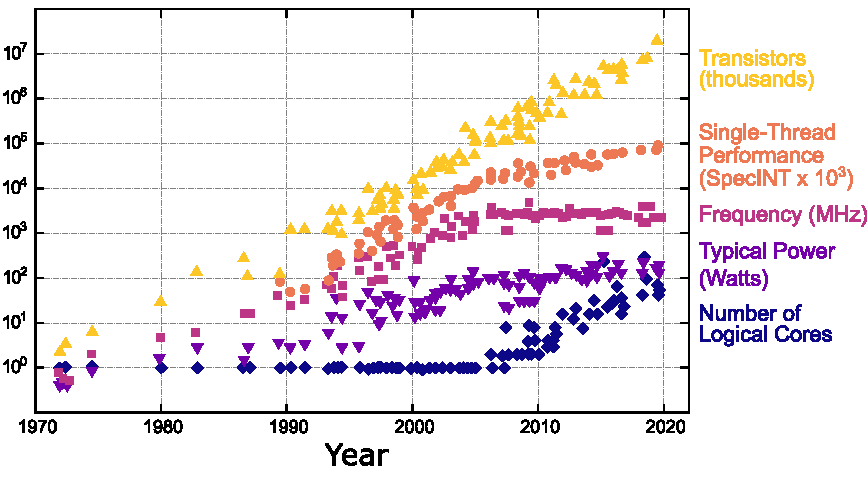
\includegraphics[width=\textwidth]{chapter_introduction/figures/moore.pdf}
        \caption[Moore's Law for Microprocessors]
        {
            The arc of Moore's law over fifty years of microprocessor development. While the number of transistors have doubled about every two years, the same cannot be said for other key figures. In particular, clock frequency and power dissipated have plateaued out since 2003. The release in 2005 by Intel of the first dual-core processor (Pentium D), and the ability to perform hyper-threading have sparked reserach into the number of logical cores per CPU. This is the ability of a single core to carry out two or more processes simultaneously. Since then, the increase in multi-threading performance compared with stagnating single-thread performance has been one of the main driving factors for multi-core processors in modern laptops. Data collected by K.\ Rupp. Adapted from a talk given by Nvidia.
        }
        \label{fig:intro:moore_law}
    \end{center}
\end{figure}
%
One of the major problematics with the \gls{CMOS}-density scaling is that as the channel length is shortened, leakge current increases because of quantum tunneling of the charge carriers through the channel. This issues has been mitigated over the last few years by adopting non-planar transistor architectures such as FinFETs~\cite{yang20045nm} and Gate-All-Around FETs~\cite{gu2011first}, but fundamental problems still remains.

Several researchers have envisioned graphene as one of the most robust materials against short-channel effects~\cite{neumaier2019integrating, chaudhry2004controlling, xie2012review, feijoo2016short,schwierz2010graphene, thiele2010modeling} and have suggested that it will be possible to integrate graphene into semiconductor manufacturing cycles in the near future. Despite its remarkable electronic and mechanic properties, several fundamental problems such as the lack of bandgap have prevented a smooth integration with integrated circuits. A candidate alternative material for this integration are \glspl{GNR}. In contrast to graphene, \glspl{GNR} are confined to one dimension, and this leads to a bandgap, making them an interesting   for semiconductor applications. From a theoretical point of view, \glspl{GNR} have attracted
much attention in the last twenty years, yet experimental evidence has remained
scarce due to the insufficient purity of fabricated GNRs. However, as a result of recent and novel developments in bottom-up synthesis, it is now possible to synthesise high-purity GNRs and atomically-precise topology that guarantees, in principle, low scattering and high device performance, as well as access to topological states.

In this work, we tackle the question of how molecular graphene nanoribbons can be integrated in low power electronic devices. We begin with a general introduction, both theoretical and experimental, to build up the groundwork of the thesis. We discuss the electronic properties of graphene, carbon nanotubes, and graphene nanoribbons and how to use them to fabricate electronic devices for high-frequency, digital and quantum applications. Since the 1D nature of graphene nanoribbons plays an important role in this research project, we present an overview of the main properties of 1D systems. In consideration
of the experimental techniques developed for this work, a chapter is dedicated to
the experimental background. We explain the fabrication recipe we have optimised to fabricate nanoelectronic devices and they instrumentation apparatus for measurements at room and \si{\milli\kelvin} temperatures. We also explore several instrumentation development we have completed and started with the goal of improving our current measurement setup. Three main research projects are then presented in detail.
Three main projects are then presented in details. We begin with the investigation of a room-temperature-operating single-electron transistor made with molecular graphene nanoribbons. This represents the first study demonstrating the physics at play in such devices. We then progress to study a chemical strategy which produces ultra-clean \gls{GNRSET}, allowing the first investigation of strong vibronic coupling in molecular graphene. Finally, we conclude by investigating two possible strategies for controlling the injection of dopants into \gls{MGNR}, i.e.\ by chemical functionalisation along the edges and by insertion of porphyrin rings carrying transition-metal ions inside the \gls{GNR} backbone.